%===================================================================================
% Chapter: Propuesta para la Extracción de Relaciones
%===================================================================================
\chapter{Propuesta para la Extracción de Relaciones}\label{chapter:relations}
\addcontentsline{toc}{chapter}{Extracción de Relaciones}

En este capítulo se hace una descripción de las técnicas empleadas para la resolución de la tarea de Extracción de Relaciones. Primeramente, se recoge un resumen del análisis de dependencias de una oración, aspecto cardinal en la propuesta realizada. Luego se describe el modelo de aprendizaje profundo propuesto, sus componentes y sus distintas variantes.


\section{Análisis de Dependencias}\label{sec:parsing}

El conocimiento de la estructura y la sintáxis que subyace en un texto en lenguaje natural puede ser de mucha ayuda en tareas típicas de NLP como la clasificación de texto, la sumarización o la extracción de relaciones. Una de las técnicas más comunes para capturar cierta estructura en las oraciones es el análisis sintáctico~(conocido comúnmente por su nombre en inglés: \emph{parsing}). En esta sección se abordará este tema, particularmente el análisis de dependencias.

Hay dos formas de describir la estructura de una oración en lenguaje natural: separando la oración en \textbf{constituyentes}~(frases), que se separan a su vez en constituyentes más pequeños; o estableciendo conexiones entre las palabras individuales~\cite{covington2001fundamental}. El significado de estas dos variantes se ilustra en las figuras \ref{fig:dep_const} y \ref{fig:dep_links} respectivamente.

\begin{figure}[h!]
	\centering
	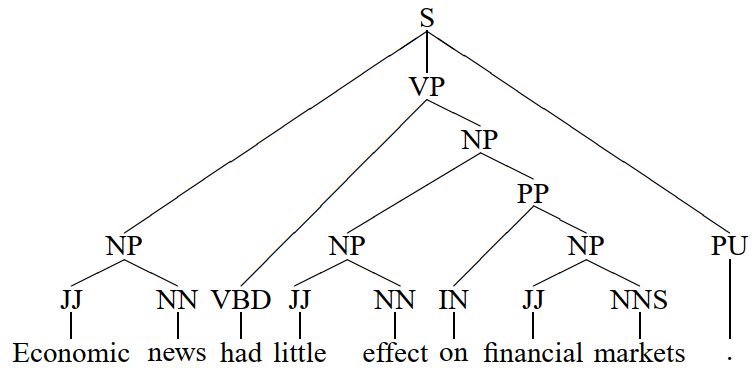
\includegraphics[width=0.8\linewidth]{Graphics/dep_const.png}
	\caption{Estructura constituyente para una oración en idioma inglés del \emph{Penn Treebank}.}\label{fig:dep_const}
\end{figure}

\begin{figure}[h!]
	\centering
	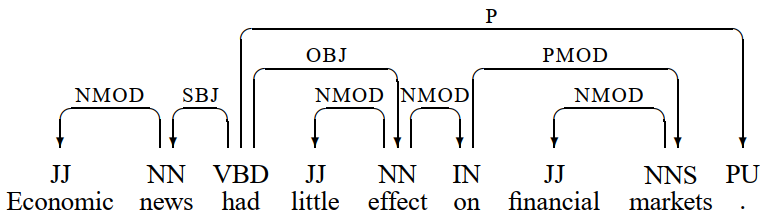
\includegraphics[width=0.8\linewidth]{Graphics/dep_links.png}
	\caption{Estructura de dependencias para una oración en idioma inglés del \emph{Penn Treebank}.}\label{fig:dep_links}
\end{figure}

La representación constituyente del lenguaje data de varios años atrás, y ha sido explotada tanto por los científicos de la computación como por lingüistas, en aras de obtener buenas representaciones del lenguaje natural. Sin embargo, la comunidad científica ha mostrado un creciente interés en los últimos años en las estructuras de dependencias como una alternativa a esta representación.

La noción fundamental de \textbf{dependencia} está basada en la idea de que la estructura sintáctica de una oración está conformada por un conjunto de relaciones binarias asimétricas entre las palabras de dicha oración~\cite{nivre2005dependency}. Siempre que se establece una relación entre dos palabras, a una de ellas se le denomina \textbf{cabecera} y a la otra \textbf{dependiente}. A continuación se listan algunos criterios que han sido propuestos para identificar una relación sintáctica entre una cabecera $H$ y un dependiente $D$, en una construcción sintáctica $C$~\cite{zwicky1985heads, richard1990english}:

\begin{enumerate}
	\item $H$ determina la categoría sintáctica de $C$, y muchas veces puede sustituir a $C$.
	
	\item $H$ determina la categoría semántica de $C$, mientras que $D$ aporta especificidad.
	
	\item $H$ es obligatoria, mientra que $D$ es opcional.
	
	\item $H$ selecciona a $D$, y determina si puede o no ser opcional.
	
	\item La forma de $D$ depende de $H$.
	
	\item La posición de $D$ en la oración se especifica con respecto a $H$.
\end{enumerate}

Estas reglas no son absolutas y contienen un mezcla de criterios variados, algunos sintácticos, otros semánticos. No existe en la literatura una noción coherente de dependencia que se corresponda con todos los distintos criterios~\cite{nivre2005dependency}.


\subsection{Grafo de dependencias}

Si se considera cada dependencia como un arco dirigido que tiene como origen a la cabecera y como destino al dependiente, la estructura de dependecias de la oración conforma un grafo dirigido $G$ cuyos nodos son los elementos léxicos del lenguaje~(\emph{tokens}). Además, el grafo subyacente de $G$ debe estar conectado, para que cada nodo esté relacionado con, al menos, otro nodo.

A esta caracterización se le imponen usualmente más restricciones. Dos de las más utilizadas en las distintas formalizaciones de gramáticas basadas en dependencias~(o simplemente, gramáticas de dependencias), son: la suposición de que cada nodo del grafo tiene \emph{indegree} $\leq 1$; y la no existencia de ciclos. Estas suposiciones, junto a la consideración de conectividad, implican que este grafo sea un árbol dirigido con una sola raíz la cual no depende de ninguna otra palabra. Esto último queda ilustrado en la figura \ref{fig:dep_tree}. A esta estructura se le denomina \textbf{árbol de dependencias}.

\begin{figure}[h!]
	\centering
	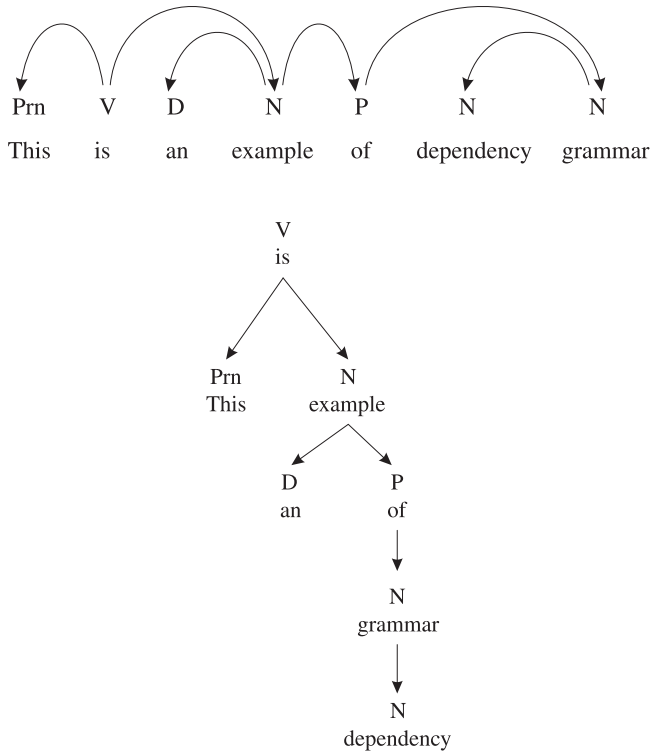
\includegraphics[width=0.7\linewidth]{Graphics/dep_tree.png}
	\caption{Estructura de dependencias para una oración en idioma inglés y árbol de dependencias.}\label{fig:dep_tree}
\end{figure}

Existen varias restricciones adicionales que se definen sobre estas estructuras y que son más debatidas. Una de las más conocidas es la restricción de \textbf{proyectividad}~\cite{hays1964dependency,lecerf1960programme,marcus1965notion}. Un grafo de dependencias satisface la restricción de proyectividad con respecto a un orden linear particular de los nodos si, por cada arco $h \rightarrow d$ y un nodo $w$, $w$ ocurre entre $h$ y $d$ en el orden lineal solo si $w$ está \textbf{dominado} por $h$~\footnote{La relación \textbf{dominar} es la clausura reflexiva y transitiva de la relación de dependencia definida por los arcos}. 

\subsection{Algoritmos para el análisis de dependencias}

Con basamento en estructuras de dependencias, disímiles algoritmos han sido propuestos para analizar el lenguaje natural.
De manera general pueden distinguirse dos enfoques diferentes que se han adoptado en la literatura: análisis orientado a gramáticas y análisis orientado a datos. 

Los trabajos pioneros en el análisis orientado a gramáticas se remontan a las propuestas de \textit{Hays} y \textit{Gaifman}, cuando en 1964 y 1965 respectivamente~\cite{hays1964dependency,gaifman1965dependency}, definieron un conjunto de reglas sobre las gramáticas de dependencias y un conjunto de condiciones que debían cumplir las relaciones de dependencia. Por su parte, los primeros intentos en realizar análisis de dependencias orientado a datos por \textit{Carroll y Charniak} en 1992~\cite{carroll1992two}, pueden considerarse también orientados a gramáticas en el sentido de que apoyaron en el formalismo de una gramática de dependencias y usaron un \emph{corpus} de datos para inducir un modelo probabilístico para la desambiguación. En esencia, usaron una Gramática Libre del Contexto Probabilística~\cite{chomsky1956three}, que estaba restringida para ser equivalente al tipo de gramáticas de \textit{Hays} y \textit{Gaifman}. 

Muchos otros trabajos se registran en la literatura relativos a propuestas de algoritmos para el análisis de dependencias~\cite{koo2008simple,mcdonald2005non,nivre2003efficient,nivre2007maltparser,socher2011parsing}. La propuesta más común se basa en algún tipo de algoritmo de programación dinámica con o sin desambiguación estadística.


\section{Modelo}\label{sec:model}

El modelo de aprendizaje profundo propuesto se apoya en el uso de RNN sobre estructuras derivadas del árbol de dependencias de la oración de entrada y las entidades señaladas para obtener una representación de la supuesta relación existente entre ellas.

\subsection{Hipótesis del Camino en el Árbol de Dependencias}

Como fue explicado en el capítulo~\ref{chapter:information_extraction}, la información más completa para resolver el problema de la extracción de relaciones se encuentra en la oración completa. Sin embargo, se maneja por muchos autores la suposición de que el árbol de dependencias de la oración de entrada condensa la información vital para resolver el problema, a la vez que desecha otras fuentes de desinformación.

\subsection{Red Neuronal}

La arquitectura definida para la resolución de ambos problemas es similar. 
La entrada de la misma se construye a partir de la secuencia de tokens de la oración, así como de los \textit{tokens} señalados.
La representación de cada token se obtiene a partir de la concatenación de \textit{embeddings} de distintas fuentes de información:

\begin{description}
	\item[Palabras:] Se utilizan \textit{embeddings} preentrenados en un corpus construido a partir de artículos de Wikipedia con contenido médico.
	Fueron entrenados utilizado el algoritmo \textbf{word2vec}\cite{word2vec} con la arquitectura \textbf{skipgram}.
	
	\item[Caracteres:] Se utilizan \textit{embeddings} obtenidos mediante una capa BiLSTM sobre los caracteres de la palabra.
	
	\item[POST-tag y Dependencia:] Se utiliza la un \textit{embedding} de la etiqueta de POS-tag de la palabra y la dependencia de la misma con su ancestro en el árbol de dependencias de la oración.
	
	\item[Etiqueta BMEWO-V y Tipo de la entidad:] Se añaden \textit{embeddings} con información relativa a la entidad a la que pertenece la palabra en cuestión.
	En este caso la etiqueta correspondiente en el sistema BMEWO-V así como el tipo de la entidad.
	
\end{description}

El procesamiento de la entrada lo realizan dos componentes: una capa BiLSTM y otra LSTM apiladas, y una capa Tree-LSTM; que operan sobre estructuras derivadas del árbol de dependencias de la oración.

\begin{description}
	\item[LSTM:] Las LSTM son un tipo de Red Neuronal Recurrente (RNN), donde en la capa oculta, las actualizaciones son reemplazadas por células de memoria especialmente diseñadas.
	Como resultado pueden ser mejores encontrando y explotando amplios rangos de dependencia en los datos~\cite{hochreiter1997long}.
	
	\item[BiLSTM:] En tareas en las que resulta conveniente tener acceso a rasgos pasados y futuros (como son las palabras que hay antes y después de otra palabra en una oración) se puede utilizar una red LSTM bidireccional, conocida como BiLSTM~\cite{graves2013speech}.
	Tradicionalmente las redes BiLSTM se entrenan usando propagación hacia atrás a través del tiempo~\cite{boden2002guide}.
	
	\item[Tree-LSTM:]
	Las redes Tree-LSTM son una generalización de la arquitectura LSTM. 
	Mientras la red LSTM tradicional computa su estado a partir de la entrada en el momento actual y el estado de la célula LSTM en el momento anterior, las Tree-LSTM lo realizan a partir del vector de entrada y los estados de una cantidad arbitraria de hijos~\cite{tai2015improved}.
	Estas redes han sido utilizadas previamente para representar estructuras sintácticas de de un oración~\cite{miwa2016end}.
	
\end{description}

Las capas recurrentes apiladas obtienen una representación de la secuencia de \textit{tokens} que aparecen en el árbol de dependencias, en el camino entre los \textit{tokens} señalados.
Entre tanto, la capa Tree-LSTM obtiene una representación del subárbol que tiene como raíz a cada \textit{token} señalado, respectivamente.

Estos tres vectores se concatentan y pasan por un clasificador constituído por una capa densa. 
En la etapa de reconocimiento, el clasificador es binario con función de activación \textit{sigmoid}.
Mientras que para la etapa de clasificación, se obtiene una distribución de probabilidades sobre el conjunto de relaciones mediante una función de activación \textit{softmax}.

La figura \ref{fig:rel_model} ilustra la arquitectura descrita para la etapa de clasificación.

\begin{figure}[h!]
	\centering
	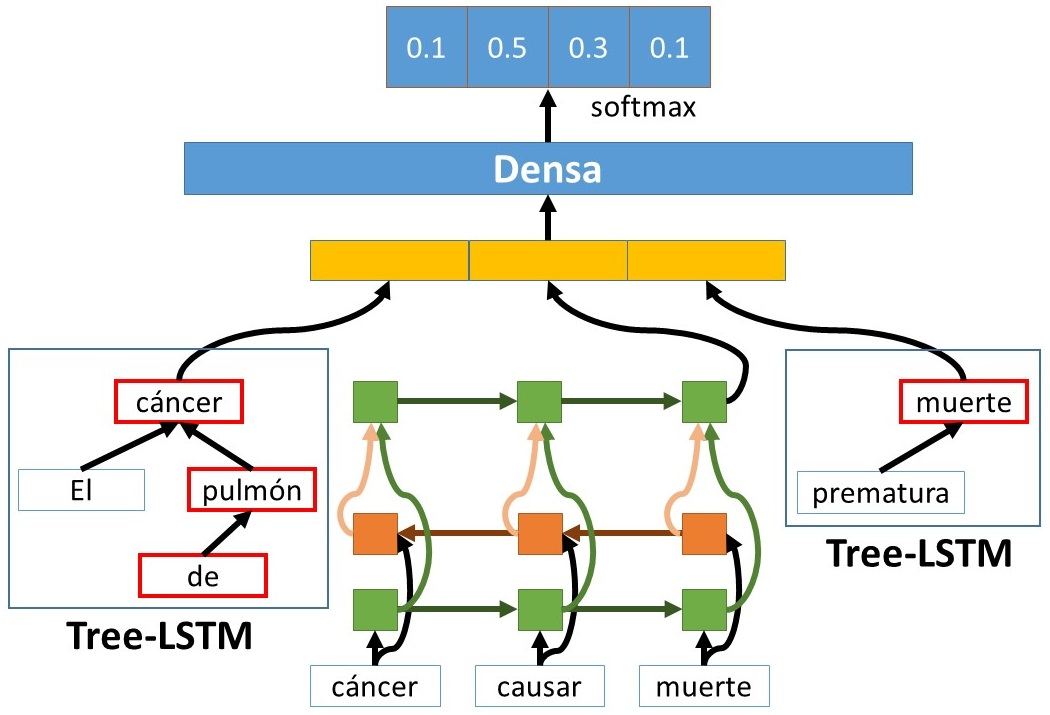
\includegraphics[width=1\linewidth]{Graphics/rel_model_class.jpg}
	\caption{Arquitectura de red utilizada. La oración de entrada es \textit{El cáncer de pulmón puede causar muerte prematura} Y las entidades en cuestión son \textit{cáncer de pulmón} y \textit{muerte}.}\label{fig:rel_model}
\end{figure}

%===================================================================================